% Where the five pilot runs sit in the cohesion--momentum landscape.
% Style after the particle-physics "lifetime atlas" idiom: logarithmic
% axes, shaded regime bands, ball-shaded markers, contoured labels.
% Compile from `docs/preprint`:  lualatex sekil/atlas.tex
\documentclass[border=3pt,tikz]{standalone}
\usepackage{pgfplots}
\usepackage{amsmath}
\usepackage[outline]{contour}
\pgfplotsset{compat=1.18}
\contourlength{1.0pt}
\tikzset{>=latex}

% Redraw the axis in front of the filled bands.
\makeatletter\newcommand{\pgfplotsdrawaxis}{\pgfplots@draw@axis}\makeatother
\pgfplotsset{axis line on top/.style={
  after end axis/.append code={\pgfplotsdrawaxis}}}

\colorlet{sweepcol}{blue!55!cyan!80!black}
\colorlet{tenscol}{red!80!black}
\colorlet{offcol}{orange!90!black}
\colorlet{obscol}{green!45!black}
\colorlet{litcol}{violet!60!black}
\colorlet{ink}{black!80}

\tikzstyle{mytick}=[ink,line width=0.5]
\tikzstyle{run}=[draw=none,ball color=#1,postaction={fill=#1,
  fill opacity=0.35,draw=#1!60!black,line width=0.12}]
\tikzset{run/.default=sweepcol}
\def\r{2.6pt}
\def\pilot[#1](#2,#3)#4{%
  \draw[run=#1] (axis cs:#2,#3) circle(\r) node#4;}

\begin{document}
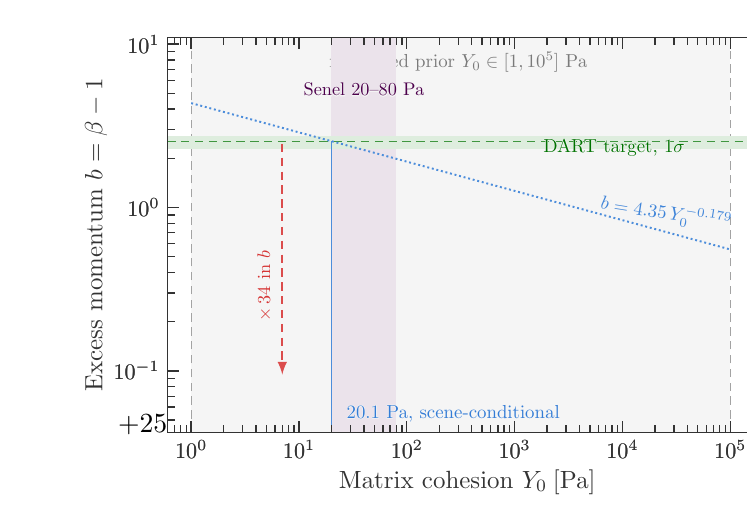
\begin{tikzpicture}
% Least-squares power law through the three sweep points, reproduced
% here from the data: b = C Y0^p with C = 4.3511, p = -0.17905.
\pgfmathsetmacro{\C}{4.3511}
\pgfmathsetmacro{\p}{-0.17905}

\begin{loglogaxis}[
  width=92mm, height=66mm,
  xmin=0.6, xmax=2.2e5, ymin=0.042, ymax=11,
  xlabel={Matrix cohesion $Y_0$\:[Pa]},
  ylabel={Excess momentum $b=\beta-1$},
  axis line style={mytick}, tick style={mytick},
  ticklabel style={scale=0.8, text=ink},
  label style={scale=0.9, text=ink},
  xlabel style={below=-2pt}, ylabel style={above=-4pt},
  axis line on top,
]

  % --- registered prior domain -----------------------------------------
  \fill[ink!5] (axis cs:1,0.042) rectangle (axis cs:1e5,11);
  \draw[densely dashed,ink!45] (axis cs:1,0.042) -- (axis cs:1,11);
  \draw[densely dashed,ink!45] (axis cs:1e5,0.042) -- (axis cs:1e5,11);
  \node[scale=0.68,text=ink!65,above] at (axis cs:300,6.1)
       {\contour{ink!5}{registered prior $Y_0\in[1,10^5]$ Pa}};

  % --- published homogeneous range -------------------------------------
  \fill[litcol!11] (axis cs:20,0.042) rectangle (axis cs:80,11);
  \node[scale=0.66,text=litcol,anchor=south] at (axis cs:40,4.4)
       {\contour{ink!5}{Senel 20--80 Pa}};

  % --- mass-adjusted DART target ---------------------------------------
  \fill[obscol!13] (axis cs:0.6,2.2948) rectangle (axis cs:2.2e5,2.7298);
  \draw[densely dashed,obscol!75] (axis cs:0.6,2.5418) -- (axis cs:2.2e5,2.5418);
  \node[scale=0.68,text=obscol,anchor=west] at (axis cs:1.6e3,2.33)
       {\contour{ink!5}{DART target, $1\sigma$}};

  % --- fitted power law -------------------------------------------------
  \addplot[domain=1:1e5,samples=60,sweepcol!70,line width=0.7pt,
           densely dotted,forget plot] {\C*x^\p};
  \node[scale=0.68,text=sweepcol!75,rotate=-9,anchor=south] at (axis cs:2.4e4,0.72)
       {$b=4.35\,Y_0^{-0.179}$};

  % --- the conditional interpolation ------------------------------------
  \draw[sweepcol!70,line width=0.5pt] (axis cs:20.13,0.042) -- (axis cs:20.13,2.5418);
  \node[scale=0.68,text=sweepcol!80,anchor=west] at (axis cs:24,0.055)
       {\contour{ink!5}{$20.1$ Pa, scene-conditional}};

  % --- the five completed runs ------------------------------------------
  \pilot[sweepcol](10,2.7480){[anchor=150,scale=0.78,text=sweepcol!55!black,
        inner sep=3pt]{\contour{white}{DY2}}}
  \pilot[sweepcol](500,1.6247){[anchor=-100,scale=0.78,text=sweepcol!55!black,
        inner sep=3.5pt]{DO1}}
  \pilot[sweepcol](5000,0.8738){[anchor=-100,scale=0.78,text=sweepcol!55!black,
        inner sep=3.5pt]{DO2}}
  \pilot[offcol](10,2.6650){[anchor=-20,scale=0.78,text=offcol!60!black,
        inner sep=3.5pt]{DN, $+25$ m}}
  \pilot[tenscol](10,0.0807){[anchor=-175,scale=0.78,text=tenscol!70!black,
        inner sep=3.5pt]{DC, tension on}}

  % --- the collapse the tension toggle produces -------------------------
  \draw[->,tenscol!70,line width=0.6pt,densely dashed]
        (axis cs:7.0,2.45) -- (axis cs:7.0,0.095);
  \node[scale=0.66,text=tenscol!80,rotate=90,anchor=south]
        at (axis cs:6.4,0.33) {$\times\,34$ in $b$};

\end{loglogaxis}
\end{tikzpicture}
\end{document}
